\section{Exponential Distribution Dataset}

\subsection{Part A: Developing Hypotheses}
Identify and collect a real-world dataset that you hypothesize follows an Exponential distribution. Please be clear about the reasoning behind your hypothesis and be specific about the source of the dataset.

We sourced a dataset from Allen Downey, a principal data scientist at PyMC and a former professor at Olin college, from his  \hyperlink{https://github.com/AllenDowney/DataExploration}{Data Exploration repository} on GitHub. This dataset possesses maternity hospital data, characterizing the intervals of births in minutes. It is a small set of timestamps through a single day, which we transformed into uni-variate observations of the inter-arrival times of consecutive births.\\

We hypothesize that birth intervals follow an Exponential distribution as this measure possess a notion of a central tendency, an average interval between births, and can at times extends to extreme values for a myriad of underlying reasons. What we see are a bunch of independent events naturally occurring a some rate throughout this day, and what is important to understand about these observations is that despite a central tendency, they are completely unrelated to the intervals between previous consecutive births. For this reason, our density function for the Exponential distribution:
$$
f(x) = \lambda e^{-\lambda x}
$$
makes a natural representation of independent events spaced out somewhat evenly. Additionally, this distribution has a decay property at further deviates from its mean in the positive direction, meaning that it can readily characterize perhaps the increasing rarity or longer intervals between births occurring, and it turn characterizes the increasing proclivity of births to occur at intervals surrounding the mean.
\newpage

\subsection{Part B: Fitting Distributions}
For this exercise, we will call each of the four different theoretical distributions (normal, uniform, power law, exponential) a ``model". Fit the dataset (i.e., estimate the model parameters) against each model (not just the one you hypothesized) using maximum likelihood estimation (or using any technique you think is appropriate; make sure to comment on the validity of your approach). This should result in a total of \textbf{4 parameter sets}. Report the estimated parameters in the following tabular format:

\begin{center}
\begin{tabular}{|c|c|c|c|c|c|}
\hline
& & \multicolumn{4}{c|}{{\bf{\em{Model}}}}\\
\hline
{{\bf{\em{Dataset}}}} & {\bf{\em{\# Observations}}} &\textbf{Normal}& \textbf{Uniform} & \textbf{Power law} & \textbf{Exponential} \\
\hline
\textbf{Dataset 4} & $n_4$ & $\mu_4, \sigma_4$ & $a_4, b_4$ & $\alpha_4, x_{\min_4}$ & $\lambda_4$ \\
\hline
\end{tabular}
\end{center}

Be sure to show the code you used to arrive at your final estimates clearly.\\
-----\\
Below are the tabulated parameter estimates for this dataset (for the full tabulation described in the original assignment TeX, see Appendix). The code in Fig. 1 was also used to arrive at our final parameter estimates for this dataset, here is the same implementation below for convenience:\\
\begin{verbatim}
def dists_fit(input_csv: str) -> tuple:
    """
    Fits the obs dataset to each model using MLE.

    :param input_csv: Path to input data to fit paramater(s) to
    :type input_csv: str
    """
    obs = pd.read_csv(input_csv).iloc[:, 0].to_numpy()

    mu = np.mean(obs)
    std = np.sqrt(np.sum((obs - mu) ** 2) / len(obs))

    a, b = obs.min(), obs.max()

    alpha = 1 + len(obs) / np.sum(np.log(obs / a))

    lamb = 1 / np.mean(obs)

    return (mu, std, a, b, alpha, lamb)
\end{verbatim}

\vspace{4pt}

\begin{center}
\begin{tabular}{|c|c|c|c|c|c|}
\hline
& & \multicolumn{4}{c|}{{\bf{\em{Model}}}}\\
\hline
{{\bf{\em{Dataset}}}} & {\bf{\em{\# Observations}}} &\textbf{Normal}& \textbf{Uniform} & \textbf{Power law} & \textbf{Exponential} \\
\hline
\textbf{Brisbane Birth Intervals} & 43 & 33.3, 29.2 & 1, 157 & 1.32, 1 & 0.0301 \\
\hline
\end{tabular}
\end{center}

\begin{center}
\textbf{Figure 13:} Parameter estimates for each model on Brisbane Birth Intervals dataset.
\end{center}

\newpage

\subsection{Part C: Comparing Real and Synthetic Data}

For each fitted distribution (there will be 4 of them for this dataset, each corresponding to a different model), generate a synthetic sample of data points equal to the sample size of the real dataset using the respective model parameters you inferred from the real dataset.\\

Compare the real vs. synthetic data distributions using methods you think are the most appropriate, including visualizations. So, for this dataset, we compare the original dataset to four synthetic datasets, all with equal number of observations, but each synthetic dataset is generated using a different model.\\

For this dataset, identify the synthetic dataset (which corresponds to a model) that is most similar to the original data in terms of its distribution.\\

Now revisit your initial hypothesis. For this dataset: Did the dataset behave as expected, or was another model (assumed distribution) a better fit to the dataset? Reflect on why the observed results may differ from your expectations.\\

We first ought to compare the samples by how well-they reflect the decaying nature of an Exponential at greater interval ranges, for which we can use a histogram:

\begin{center}
  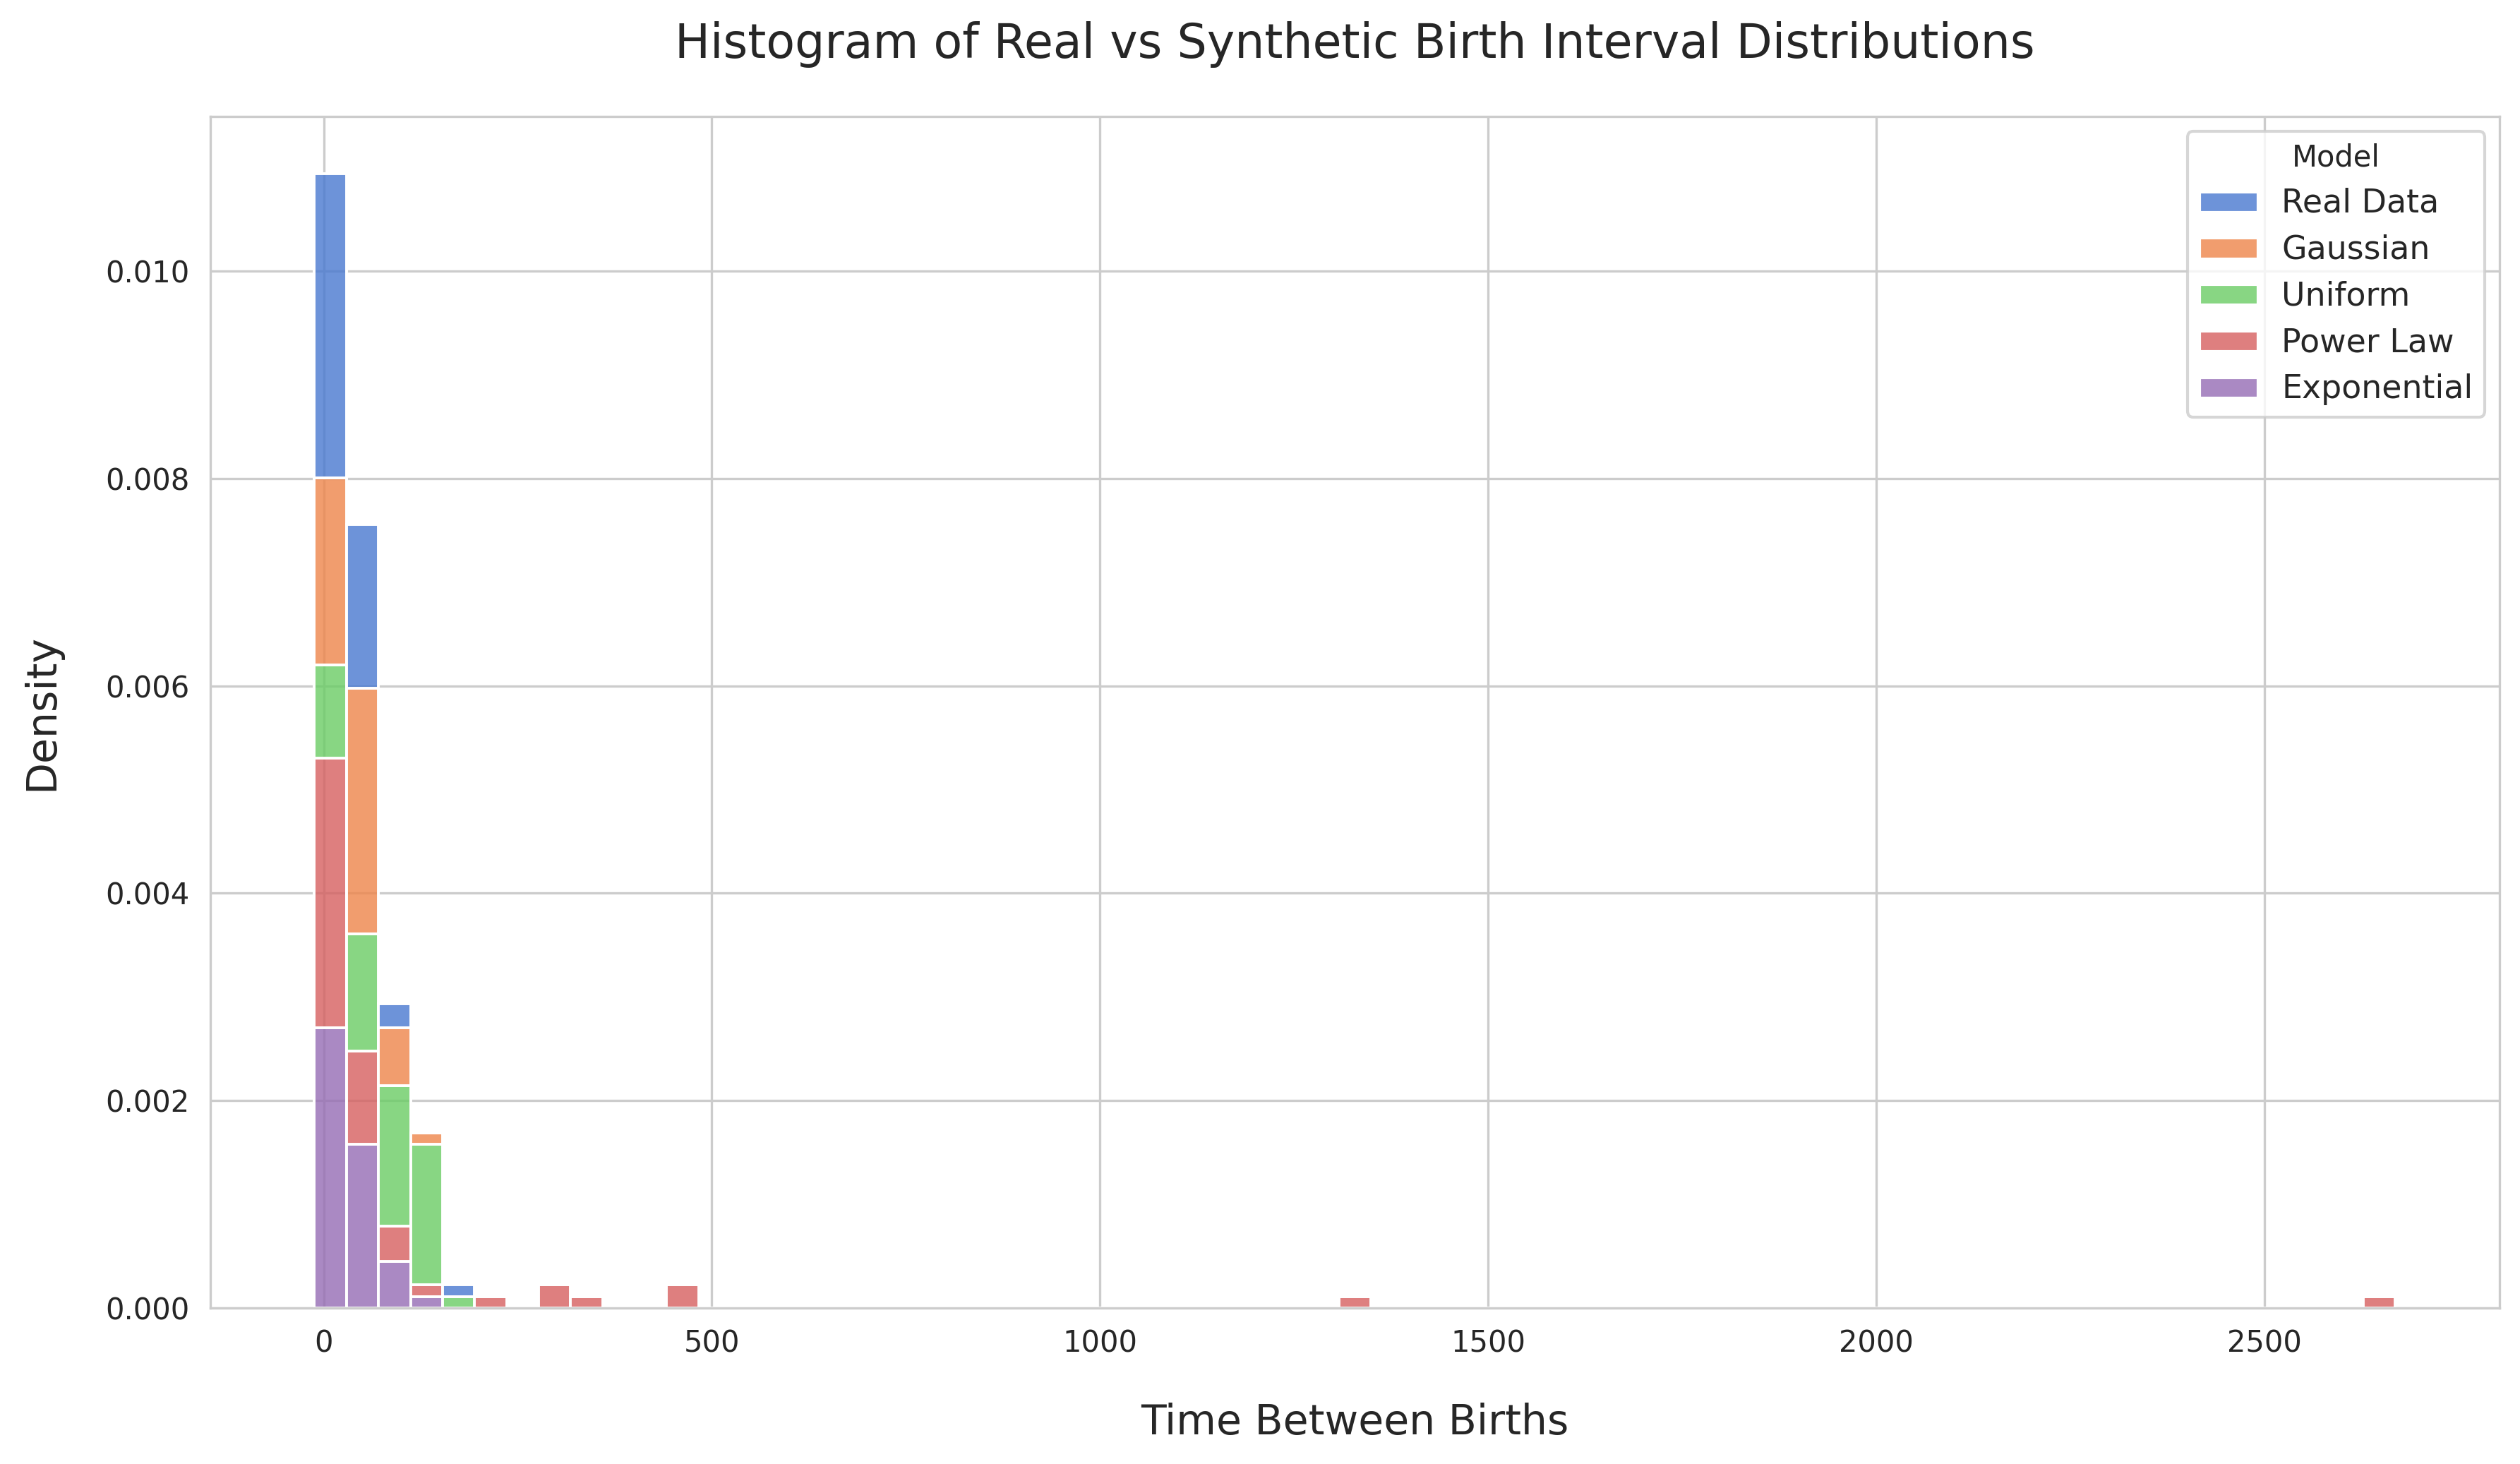
\includegraphics[width=0.95\textwidth]{figures/exponential/histogram.png}
  
  \textbf{Figure 14:} Histogram of Real vs Synthetic Distributions on Birth Intervals dataset.
\end{center}

Viewing how the mass is distributed was challenging for overlapping distributions, so we chose to stack them, and it is clear visually that for where the mass is concentrated in the real dataset, we see more mass distributed in the same spot for the Power Law Distribution and the Exponential distribution. It is also apparent that the Power Law distribution is still trying to fit to extreme values in the data, suggesting that while a strong choice, it may not be the best option for representing a decay pattern at extremes. The other two datasets are quite unsuitable in this case and are showcase their own idiosyncrasies while somewhat adhere to the structure of the Birth Intervals dataset.\\

We produced a K-S test below to gain a more concrete understanding of how the Power Law distribution and the Exponential distribution compare in this context:

\begin{center}
\begin{tabular}{|c|c|c|c|}
\hline
\textbf{Distribution} & \textbf{K-S Statistic} & \textbf{p-value} & \textbf{Significant} \\
\hline
Gaussian & 0.28 & 0.070 & No \\
\hline
Uniform & 0.51 & 1.73 $\times 10^{-5}$ & Yes \\
\hline
Power Law & 0.30 & 0.039 & Yes \\
\hline
Exponential & 0.12 & 0.938 & No \\
\hline
\end{tabular}
\end{center}

\begin{center}
\textbf{Figure 15:} Kolmogorov-Smirnov test results between the Birth Intervals dataset and synthetic samples.
\end{center}

Surprisingly, the K-S test told us that there is actually much higher disagreement than we could discern from the histogram alone between the real data and the Power Law model with a significant p-value of 0.039, and even more surprisingly, the Gaussian, while not as in agreement with the data as the Exponential, agrees more with the real data than the Power Law distribution, which perhaps makes sense when you reduce them both to distributions that prioritize decay away from the center.\\

From these visualizations, we can make a confident claim that the dataset produce by the Exponential distribution is most similar to the real dataset. This was the expected behavior for this data, and in fact the fit and visualization showed with much greater clarity how important the general notions of a distribution are to how it is characterized, and specifically how it is differentiated from others. Two distributions like Power Law and Exponential can look very similar, but there is nuance that distances them greater than may be readily apparent.
